\exer{[EQD-001]}
\setcounter{numques}{0}~\\

\subsection*{Autour de la dynamique gravitationnelle}

\subsubsection*{Présentation}
Modéliser les interactions physiques entre un grand nombre de constituants mène à l'écriture de systèmes différentiels pour lesquels, en dehors de quelques situations particulières, il n'existe aucune solution analytique. Les problèmes de dynamique gravitationnelle et de dynamique moléculaire en sont deux exemples. Afin d'analyser le comportement temporel de tels systèmes, l'informatique peut apporter une aide substantielle en permettant leur simulation numérique. L'objet de ce sujet est l'étude de solutions algorithmiques en vue de simuler une dynamique gravitationnelle afin, par exemple, de prédire une éclipse ou le passage d'une comète.

\subsubsection*{Quelques fonctions utilitaires}

\question{}Donner la valeur des expressions python suivantes :
\begin{itemize}
\item $[1, 2, 3] + [4, 5, 6]$
\item $2 * [1, 2, 3]$
\end{itemize}


\question{} Écrire une fonction python $smul$ à deux paramètres, un nombre et une liste de nombres, qui multiple chaque élément de la liste par le nombre et renvoie une deuxième liste sans modifier la première. 
Par exemple, \textit{smul(2, [1, 2, 3])} renvera \textit{[2, 4, 6]}.

\question{} Déterminer la complexité de cet algorithme en fonction de la taille de la liste.


\subsection*{Étude de schémas numériques}

Soient $y$ une fonction de classe $\mathcal{C}^2$ sur $\R$ et $t_{min}$ et $t_{max}$ deux réels tels que $t_{min} < t_{max}$. On note $I$ l'intervalle $\left[t_{min}, t_{max}\right]$. 
On s'intéresse à une équation différentielle du second ordre de la forme :

\begin{align}\label{eqn1}
\forall t \in I && y''(t)=f(y(t)),
\end{align}

où $f$ est une fonction donnée, continue sur $\R$. De nombreux systèmes physiques peuvent être décrits par une
équation de ce type.

On suppose connues les valeurs $y_0 = y(t_{min})$ et $z_0 = y'(t_{min})$. 

\subsubsection*{Mise en forme du problème}

Pour résoudre numériquement l'équation différentielle \eqref{eqn1}, on introduit la fonction $z$ : $I\to \R$ définie par 

\begin{equation}
\forall t\in I, z(t)=y'(t).
\end{equation}

On considère l'équation : 

\begin{equation}\label{eqn4}
Y'=F(Y,t)
\end{equation}

\question{} Pour quelle variable $Y$ et quelle fonction $F$, l'équation \eqref{eqn1} peut se mettre sous la forme de l'équation \eqref{eqn4} ?


Soit $n$ un entier strictement supérieur à 1 et $J_n=\llbracket 0,n-1 \rrbracket$.
On pose $h=\dfrac{t_{max}-t_{min}}{n-1}$ et $\forall i \in J_n$, $t_i=t_{min}+i\cdot h$. On peut montrer que, pour tout entier $i\in \llbracket 0,n-2 \rrbracket$,

\begin{equation}\label{eqn3}
\displaystyle
Y(t_{i+1})=Y(t_i)+\int_{t_i}^{t_{i+1}}Y'(t)dt
\end{equation}


La suite du problème exploite les notations introduites dans cette partie et présente deux méthodes numériques
dans lesquelles l'intégrale précédente est remplacée par une valeur approchée.

\subsubsection*{Schéma d'Euler explicite}

Dans le schéma d'Euler explicite, chaque terme sous le signe intégrale est remplacé par sa valeur prise en la borne inférieure.


\question{} Ecrire une fonction $euler(F, tmin, tmax, Y_0, n)$ qui renvoie deux listes de nombres correspondant aux valeurs associées aux suites $\left(y_i\right)_{i\in J_n}$, $\left(z_i\right)_{i\in J_n}$ ainsi que la liste du temps $\left(t_i\right)_{i\in J_n}$.

\bigskip{}

Pour illustrer cette méthode, on considère l'équation différentielle, 

\begin{equation}\label{eqn5}
\forall t\in I,\quad y''(t) = -\omega^2y(t)
\end{equation}

dans laquelle $\omega$ est un nombre réel.

\question{} Expliciter en langage \texttt{Python} la fonction $F(Y,t)$ et la fonction $f(y)$ qui permettront de mettre en oeuvre ce problème.

\bigskip

La mise en oeuvre de la méthode d'Euler explicite génère le résultat graphique donné figure \ref{fig1}. Dans
un système d'unités adapté, les calculs ont été menés en prenant $y_0 = 3$, $z_0 = 0$, $t_{min} = 0$, $t_{max} = 3$, $\omega = 2\pi$ et $n = 100$.

\question{} \'Ecrire la suite d'instructions permettant à partir de la fonction $F$ et après avoir défini la fonction $euler$ de la mettre en oeuvre et produire le tracé de la figure \ref{fig1}. 


\begin{figure}[!h]
\begin{center}
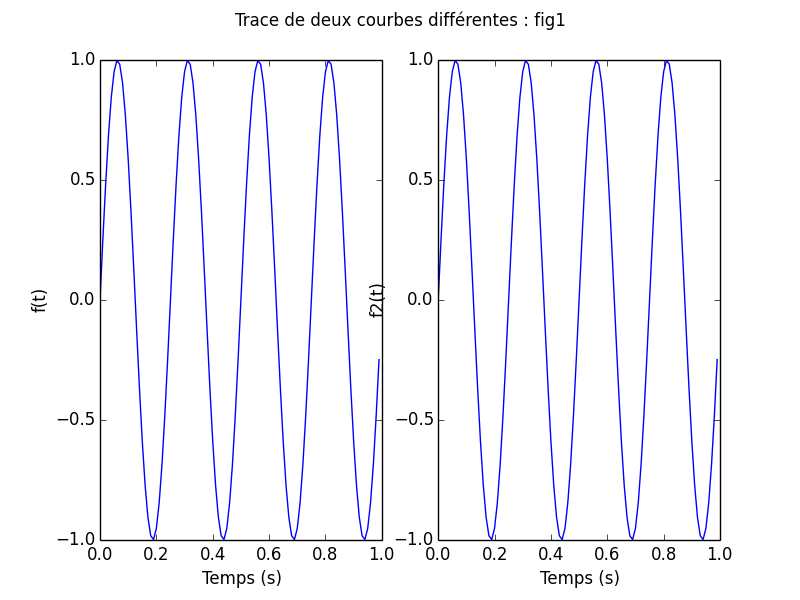
\includegraphics[width=0.7\textwidth]{fig1.png}
\caption{Portrait de phase avec la méthode d'Euler\label{fig1}}
\end{center}
\end{figure}


\subsubsection*{Schéma de Verlet}


%

Le physicien français Loup Verlet a proposé en 1967 un schéma numérique d'intégration d'une équation de la forme \eqref{eqn1} dans lequel, en notant $f_i=f(y_i)$ et $f_{i+1}=f(y_{i+1})$, les relations de récurrence s'écrivent, pour tout entier $i\in \llbracket 0,n-2 \rrbracket$ : 

\begin{align}\label{eqn6}
\displaystyle
y_{i+1}=y_i+hz_i+\dfrac{h^2}{2}f_i && \textrm{et} && z_{i+1}=z_i+\dfrac{h}{2}\left(f_i+f_{i+1}\right).
\end{align}

\question{}
Écrire une fonction $verlet(f, tmin, tmax, Y_0, n)$ qui renvoie deux listes de nombres correspondant aux valeurs associées aux suites $\left(y_i\right)_{i\in J_n}$ et $\left(z_i\right)_{i\in J_n}$, ainsi que la liste du temps $\left(t_i\right)_{i\in J_n}$.

\bigskip

On reprend l'exemple de l'oscillateur harmonique défini par l'équation~\eqref{eqn5} et on compare les résultats obtenus à l'aide des schémas d'Euler et de Verlet.


\question{} \'Ecrire la suite d'instructions permettant à partir de la fonction $f$ et après avoir défini la fonction $verlet$ de la mettre en oeuvre et produire le tracé de la figure \ref{fig2}. 

\subsubsection*{Comparaison qualitative des schémas numériques.}

On rappelle que l'énergie pour un tel oscillateur est proportionnelle à : 
\begin{equation*}
  \mathcal{E} = \dfrac{1}{2}(y')^2 + \dfrac{\omega^2}{2}y^2.
\end{equation*}

\question{} Conclure sur la stabilité des deux schémas numériques.

\begin{figure}[!h]
\begin{center}
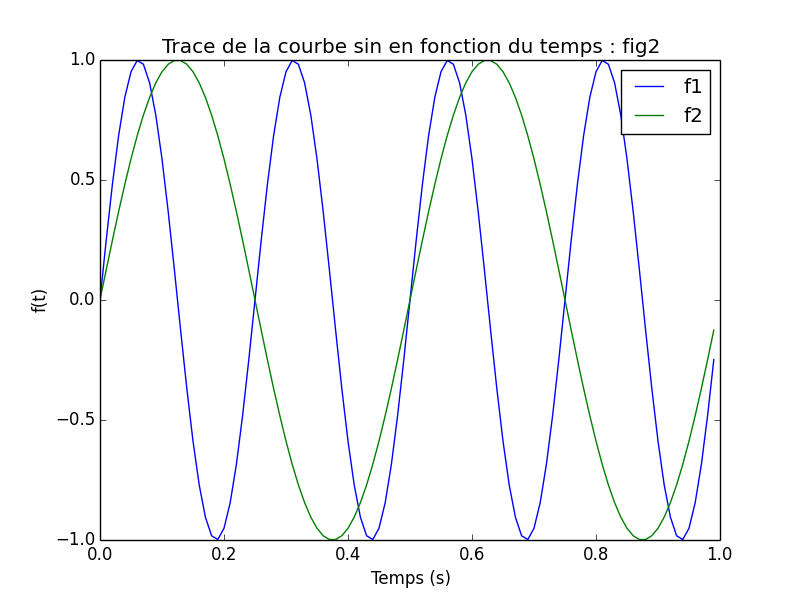
\includegraphics[width=0.7\textwidth]{fig2.png}
\caption{Portrait de phase avec la méthode de Verlet\label{fig2}}
\end{center}
\end{figure}